\section{SUBPLOT Subplot Function}

\subsection{Usage}

This function divides the current figure into a 2-dimensional
grid, each of which can contain a plot of some kind.  The function
has a number of syntaxes.  The first version 
\begin{verbatim}
   subplot(row,col,num)
\end{verbatim}
which either activates subplot number \verb|num|, or 
sets up a subplot grid of size \verb|row x col|, and then
activates \verb|num|. You can also set up subplots that cover multiple
grid elements
\begin{verbatim}
   subplot(row,col,[vec])
\end{verbatim}
where \verb|vec| is a set of indexes covered by the new subplot.
Finally, as a shortcut, you can specify a string with three
components
\begin{verbatim}
   subplot('mnp')
\end{verbatim}
or using the alternate notation
\begin{verbatim}
   subplot mnp
\end{verbatim}
where \verb|m| is the number of rows, \verb|n| is the number of columns
and \verb|p| is the index.  You can also specify the location of the
subplot explicitly using the syntax
\begin{verbatim}
   subplot('position',[left bottom width height])
\end{verbatim}

\subsection{Example}

Here is the use of \verb|subplot| to set up a \verb|2 x 2| grid of plots
\begin{verbatim}
--> t = linspace(-pi,pi);
--> subplot(2,2,1)
--> plot(t,cos(t).*exp(-2*t));
--> subplot(2,2,2);
--> plot(t,cos(t*2).*exp(-2*t));
--> subplot(2,2,3);
--> plot(t,cos(t*3).*exp(-2*t));
--> subplot(2,2,4);
--> plot(t,cos(t*4).*exp(-2*t));
\end{verbatim}


\centerline{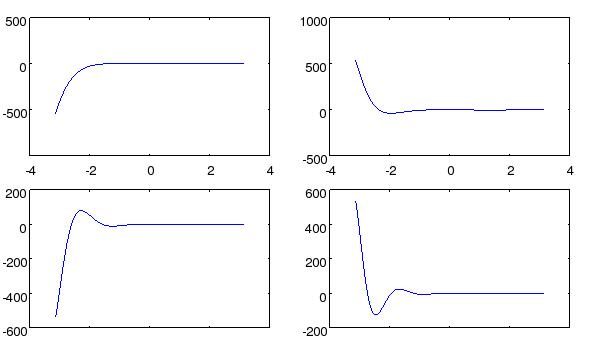
\includegraphics[width=8cm]{subplot1}}

Here we use the second form of \verb|subplot| to generate one subplot
that is twice as large.
\begin{verbatim}
--> t = linspace(-pi,pi);
--> subplot(2,2,[1,2])
--> plot(t,cos(t).*exp(-2*t));
--> subplot(2,2,3);
--> plot(t,cos(t*3).*exp(-2*t));
--> subplot(2,2,4);
--> plot(t,cos(t*4).*exp(-2*t));
\end{verbatim}


\centerline{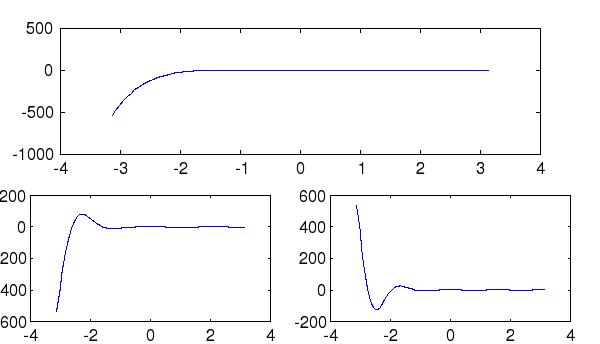
\includegraphics[width=8cm]{subplot2}}

Note that the subplots can contain any handle graphics objects,
not only simple plots.
\begin{verbatim}
--> t=0:(2*pi/100):(2*pi);
--> x=cos(t*2).*(2+sin(t*3)*.3);
--> y=sin(t*2).*(2+sin(t*3)*.3);
--> z=cos(t*3)*.3;
--> subplot(2,2,1)
--> plot(t,x);
--> subplot(2,2,2);
--> plot(t,y);
--> subplot(2,2,3);
--> plot(t,z);
--> subplot(2,2,4);
--> tubeplot(x,y,z,0.14*sin(t*5)+.29,t,10)
--> axis equal
--> view(3)
\end{verbatim}


\centerline{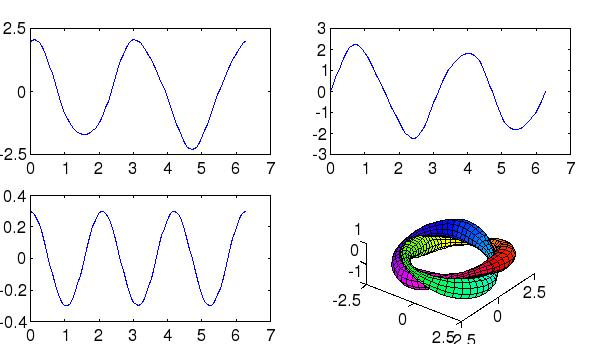
\includegraphics[width=8cm]{subplot3}}

